%% LyX 1.6.5 created this file.  For more info, see http://www.lyx.org/.
%% Do not edit unless you really know what you are doing.
\documentclass[11pt,english,ngerman,pointlessnumbers, abstraction, headsepline]{scrreprt}
\usepackage{lmodern}
\renewcommand{\sfdefault}{lmss}
\renewcommand{\ttdefault}{lmtt}
\usepackage[T1]{fontenc}
\usepackage[latin9]{inputenc}
\usepackage{listings}
\usepackage[a4paper]{geometry}
\geometry{verbose,tmargin=3cm,bmargin=3cm,lmargin=3cm,rmargin=2.75cm,headheight=1cm,headsep=0.666cm,footskip=1cm}
\setcounter{secnumdepth}{3}
\setcounter{tocdepth}{3}
\setlength{\parskip}{\medskipamount}
\setlength{\parindent}{0pt}
\usepackage{babel}

\usepackage{verbatim}
\usepackage{float}
\usepackage{url}
\usepackage{graphicx}
\usepackage{setspace}
\setstretch{1.4}
\usepackage[unicode=true, 
 bookmarks=true,bookmarksnumbered=false,bookmarksopen=true,bookmarksopenlevel=2,
 breaklinks=false,pdfborder={0 0 0},backref=false,colorlinks=false]
 {hyperref}
\hypersetup{pdftitle={Warum die Welt eine Scheibe ist},
 pdfauthor={Max Mustermann}}
 
\makeatletter

%%%%%%%%%%%%%%%%%%%%%%%%%%%%%% LyX specific LaTeX commands.
\providecommand{\LyX}{L\kern-.1667em\lower.25em\hbox{Y}\kern-.125emX\@}
%% Because html converters don't know tabularnewline
\providecommand{\tabularnewline}{\\}

%%%%%%%%%%%%%%%%%%%%%%%%%%%%%% Textclass specific LaTeX commands.
\newenvironment{lyxcode}
{\par\begin{list}{}{
\setlength{\rightmargin}{\leftmargin}
\setlength{\listparindent}{0pt}% needed for AMS classes
\raggedright
\setlength{\itemsep}{0pt}
\setlength{\parsep}{0pt}
\normalfont\ttfamily}%
 \item[]}
{\end{list}}

%%%%%%%%%%%%%%%%%%%%%%%%%%%%%% User specified LaTeX commands.
%% Flexibles Seitenlayout
\usepackage[automark]{scrpage2}

%% Mehrspaltenlayout erm�glichen
\usepackage{multicol}

%% Unterst�tzung f�r Farben
\usepackage{color}

%% Sch�nere Tabellen
\usepackage{booktabs, longtable}

%% Sch�nerer Blocksatz
\usepackage{microtype}

%% Mehr Platz zwischen �berschrift und Tabelle
\newcommand{\@ldtable}{}
\let\@ldtable\table
\renewcommand{\table}{ %
    \setlength{\@tempdima}{\abovecaptionskip} %
    \setlength{\abovecaptionskip}{\belowcaptionskip} %
    \setlength{\belowcaptionskip}{\@tempdima} %
    \@ldtable %
}

%% Verschiedene Symbole und Zeichen wie (c), �
\usepackage{textcomp}

%% Fehlerkorrektur f�r Marginalien
\usepackage{fixltx2e, mparhack}

%% Deutsche Kurzfassung und englisches Abstract auf eine Seite
\renewenvironment{abstract}{
    \@beginparpenalty\@lowpenalty
        \begin{center}
            \normalfont\sectfont\nobreak\abstractname
        \end{center}
    \@endparpenalty\@M
}{
    \par
}

%% Alle Seiten vor dem Inhaltsverzeichnis sind r�misch nummeriert
\pagenumbering{roman}
\let\myTOC\tableofcontents
\renewcommand\tableofcontents{
    \begin{spacing}{1.1}
    \myTOC
    \end{spacing}
    \clearpage
    \pagenumbering{arabic}
}

%% Kopfzeile um Logo erg�nzen
\clearscrheadfoot
\ohead{\\\headmark}
\ihead{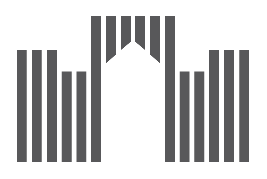
\includegraphics[scale=0.25]{pics/FH-Logo-only-gray}}%\pagemark}
\ofoot[\pagemark]{\pagemark}

%% Randnotizen anpassen
\setlength{\marginparwidth}{22mm}
\let \oldmarginpar = \marginpar
\renewcommand{\marginpar}[1]{%
    \-\oldmarginpar[\raggedleft\footnotesize\sf #1]%
        {\raggedright\footnotesize\sf #1%
    }}

%% Zitate am Kapitelanfang
\usepackage{epigraph}
\setlength{\epigraphwidth}{9cm}

%% Code-Block-Formatierung
\lstdefinestyle{default}{ %
    backgroundcolor={\color[rgb]{0.95,0.95,0.95}}, %
    basicstyle={\small\ttfamily}, %
    breaklines=true, %
    frame=l, %
    language={[Sharp]C}, %
    lineskip=-0.1pt, %
    numbers=left, %
    rulecolor={\color[rgb]{0.5,0.5,0.5}}, %
    xleftmargin={0.75cm}, %
    xrightmargin={0cm} %
}

\makeatother

\begin{document}
\titlepage

\begin{center}

\includegraphics[width=8cm]{pics/Technische_Hochschule_Brandenburg_Logo}\vspace{0.5cm}

\par\end{center}

\noindent \begin{center}
\textsf{\textbf{\Large Fachbereich Informatik und Medien}}\\
\textsf{\large }\\
\vspace{1cm}

\par\end{center}

\noindent \begin{center}
\textsf{\textbf{\huge MASTERARBEIT}}\textsf{}\\
\textsf{}\\
\textsf{\Large Warum die Welt eine Scheibe ist}
\par\end{center}{\Large \par}

\vspace{2cm}


\noindent \begin{center}
{\huge }\begin{tabular}{rl}
Vorgelegt von: & Muster Klausmann\tabularnewline
am: & 01.01.2009\tabularnewline
\end{tabular}
\par\end{center}{\huge \par}

\vspace{1cm}


\noindent \begin{center}
zum \\
Erlangen des akademischen Grades\textsf{}\\
\textsf{\smallskip{}
}
\par\end{center}

\noindent \begin{center}
\textsf{\textbf{\huge MASTER OF SCIENCE}}\textsf{\textbf{\LARGE }}\\
\textsf{\textbf{(M.Sc.)}}
\par\end{center}

\noindent \begin{center}
\medskip{}
\begin{tabular}{rl}
Erstbetreuer: & Bruno Giordano\tabularnewline
Zweitbetreuer: & Prof. Jens Haberblatt\tabularnewline
\end{tabular}
\par\end{center}

\newpage{}

%
\begin{comment}
leere Seite nach dem Titelblatt

dann Aufgabenstellung
\end{comment}
{}

\selectlanguage{ngerman}%
\tableofcontents{}

\pagestyle{scrheadings}    %Kopfzeile ein


\chapter{Aufgabenstellung}

In einem Experiment wurden Eyetracking-Daten erhoben, bei denen die Versuchspersonen drei verschiedene Versuche durchf\"uhren sollten. Dabei sollten die Versuchsperson mit den Augen einem Punkt folgen, der eine spezielle Figur zeichnete. Diese Figuren sind eine liegende acht und eine horizontale Linie.

\begin{itemize}
	\item Der erste Versuch ist die liegende acht langsam (acht Sekunden f\"ur einen Durchlauf).
	\item Der zweite Versuch ist die liegende acht schnell (vier Sekunden f\"ur einen Durchlauf).
	\item Der dritte Versuch ist die horizontale Linie (vier Sekunden f\"ur einen Durchlauf).
\end{itemize}

F\"ur jeden Versuch wurden zwei Messungen gemacht und f\"ur die liegende Acht langsam wurde zus\"atzlich ein Probedurchlauf gemacht.
Die Aufgabe besteht darin die Versuchspersonen zu gruppieren (clustern). Dabei sollen mit Hilfe der erhobenen Daten Merkmale gefunden werden, die es erm\"oglichen Gruppen zu bilden.
Zu dem Ergebnis geh\"oren folgende Bestandteile:

\begin{enumerate}
	\item Die Cluster
	\item Die Beschreibungen der Cluster
	\item Die Merkmale, die erzeugt wurden
\end{enumerate}

Die Aufgabe wird seit dem 30.11.2016 bearbeitet.
\chapter{Datenbeschreibung}
Die Daten umfassen f\"ur 134 Versuchspersonen jeweils eine Datei mit Daten zu den gemessenen Blickpositionen (Blickdatei) und eine Datei mit den Positionsdaten des Zielpunktes (Targetdatei).\\
Die Tabelle \ref{tab:AttrBlickdatei} zeigt die Attribute der Blickdateien:

\begin{table}[H]
	\caption{\label{tab:AttrBlickdatei}Attribute Blickdatei}
	
	
	\noindent \centering{}
	\bgroup
	\def\arraystretch{2}  %  1 ist der Standardwert
	\begin{tabular}{|l|l|}
		\hline 
		\textbf{Attribut} & \textbf{Wert}\\
		\hline \hline
		Zeitstempel & Ganze Zahl positiv --> Zeitreihen\\
		\hline
		Blick linkes Auge x-Koordinate & Flie\ss{}kommazahl \\
		\hline
		Blick linkes Auge y-Koordinate & Flie\ss{}kommazahl \\
		\hline
		Pupillengr\"o\ss{}e linkes Auge & Kann ignoriert werden \\
		\hline
		Position linkes Auge vor Eyetracker x-Koordinate & Kann ignoriert werden \\
		\hline
		Position linkes Auge vor Eyetracker y-Koordinate & Kann ignoriert werden \\
		\hline
		Entfernung linkes Auge vor Eyetracker & Kann ignoriert werden \\
		\hline
		Blick rechtes Auge x-Koordinate & Flie\ss{}kommazahl \\
		\hline
		Blick rechtes Auge y-Koordinate & Flie\ss{}kommazahl \\
		\hline
		Pupillengr\"o\ss{}e rechtes Auge & Kann ignoriert werden \\
		\hline
		Position rechtes Auge vor Eyetracker x-Koordinate & Kann ignoriert werden \\
		\hline
		Position rechtes Auge vor Eyetracker y-Koordinate & Kann ignoriert werden \\
		\hline
		Entfernung rechtes Auge vor Eyetracker & Kann ignoriert werden \\
		\hline
	\end{tabular}
	\egroup
\end{table}

Die Tabelle \ref{tab:AttrTargetdatei} zeigt die Attribute der Targetdateien:

\begin{table}[H]
	\caption{\label{tab:AttrTargetdatei}Attribute Targetdatei}
	
	
	\noindent \centering{}
	\bgroup
	\def\arraystretch{2}  %  1 ist der Standardwert
	\begin{tabular}{|l|l|}
		\hline 
		\textbf{Attribut} & \textbf{Wert}\\
		\hline \hline
		Zeitstempel & Ganze Zahl positiv --> Zeitreihen\\
		\hline
		t\_soll & Kann ignoriert werden \\
		\hline
		t\_ist & Kann ignoriert werden \\
		\hline
		pix\_x & Flie\ss{}kommazahl \\
		\hline
		pix\_y & Flie\ss{}kommazahl \\
		\hline
		deg\_x & Kann ignoriert werden \\
		\hline
		deg\_y & Kann ignoriert werden \\
		\hline
	\end{tabular}
	\egroup
\end{table}

Eine Blickdatei enth\"alt zus\"atzlich zu den erfassten Blickpositionen noch Eventeintr\"age. Diese Eventeintr\"age haben auch einen Zeitstempel und unterteilen die Datei in verschiedene Phasen des Experiments. Dabei weisen die Eventeintr\"age eine typische Reihenfolge auf.
Die Tabelle \ref{tab:Events} Eventeintr\"age k\"onnen auftreten:

\begin{table}[H]
	\caption{\label{tab:Events}Eventeintr\"age}
	
	
	\noindent \centering{}
	\bgroup
	\def\arraystretch{2}  %  1 ist der Standardwert
	\begin{tabular}{|p{7.5cm}|p{7.5cm}|}
		\hline 
		\textbf{Event} & \textbf{Bedeutung}\\
		\hline \hline
		START:PursuitTask & Beginn der kompletten Aufgabe (Alle Versuche)\\
		\hline
		PURSUIT:Cycles=1:Trajectory=lying\_eight:\newline T=8 & Markierung eines Versuchs,\newline
		Angabe der Zyklen, \newline
		Versuch und Dauer in Sekunden \\
		\hline
		Fixcross & Kalibrierung \\
		\hline
		Cycle:1:START & Beginn der Figur \\
		\hline
		Cycle:1:STOP & Ende der Figur \\
		\hline
		PURSUIT\_FINISHED:Cycles=1:Trajectory\newline=lying\_eight:T=8 & Markierung des Endes eines Versuchs, \newline
		Angabe der Zyklen, \newline Versuch und Dauer in Sekunden \\
		\hline
		STOP:PursuitTask & Ende der kompletten Aufgabe (Alle Versuche) \\
		\hline
	\end{tabular}
	\egroup
\end{table}

Abbildung \ref{fig:liegendeAcht} zeigt, wie die Eventeintr\"age den Versuch liegende acht langsam in verschiedene Phasen aufteilen.

\begin{figure}[H]
	\noindent \begin{centering}
		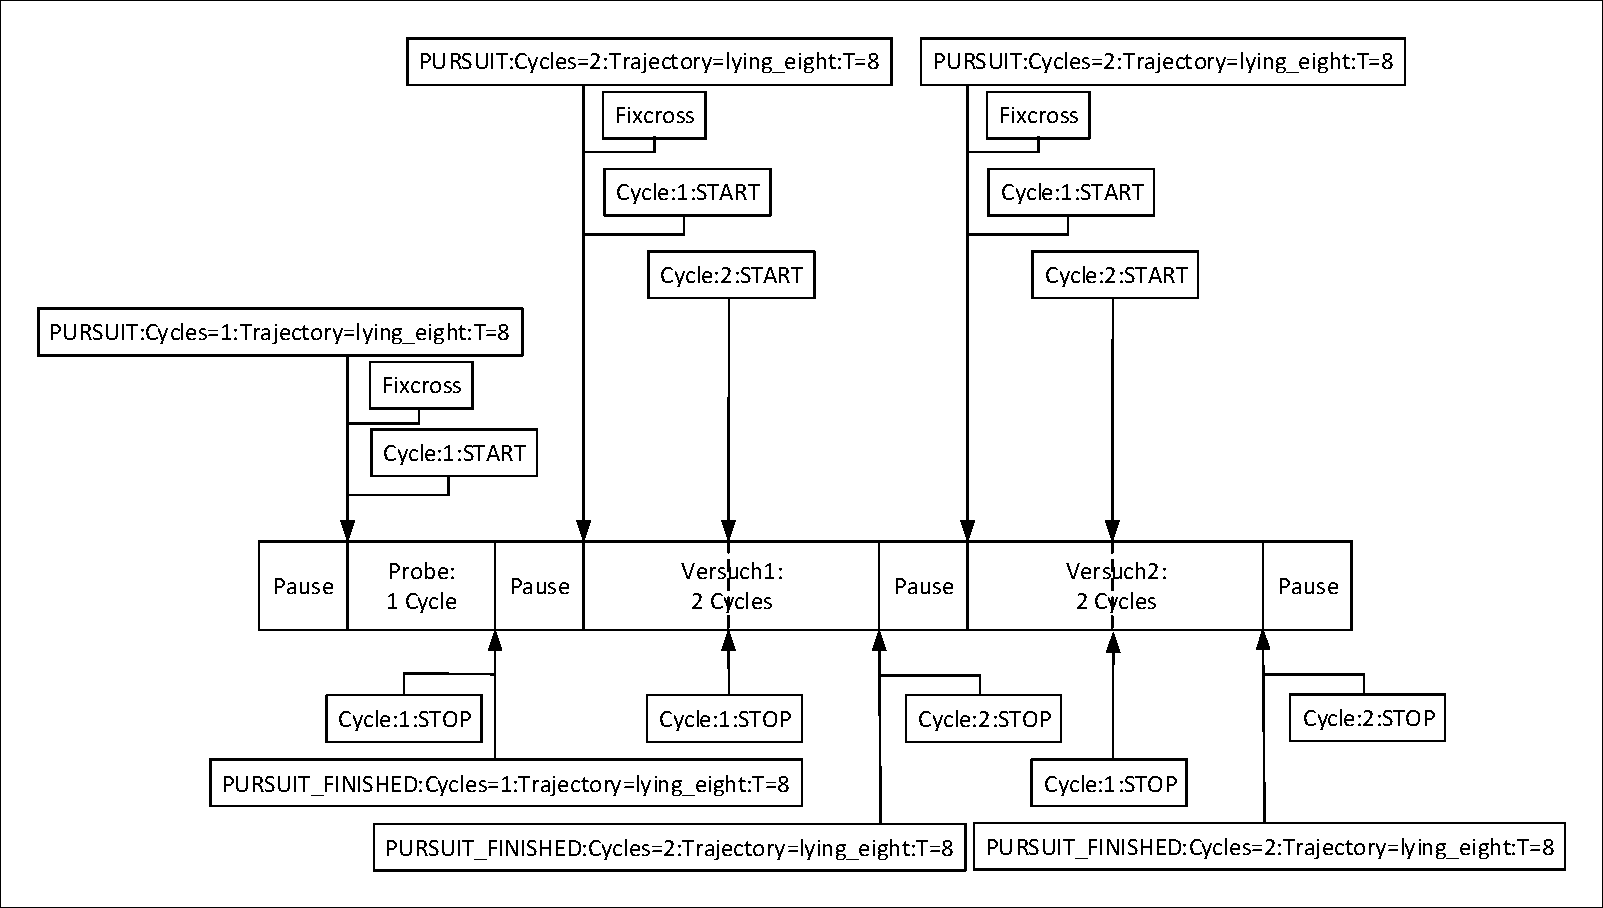
\includegraphics[width=15cm]{pics/Phasen-liegende-Acht.pdf}
		\par\end{centering}
	\caption{\label{fig:liegendeAcht}Phasen liegende Acht}
\end{figure}
\chapter{Untersuchung der Daten}

Um ein besseres Verst\"andnis f\"ur die Daten zu bekommen haben wir diese zun\"achst so zerlegt, dass die Blickdaten in kleineren Dateien gespeichert wurden, die nur noch jeweils die Daten f\"ur einen Versuch enthalten. Die Targetdateien wurden ebenfalls so zerlegt, dass kleine Dateien entstanden, die die Daten f\"ur einen Versuch pro Versuchsperson enthalten.
Die Daten wurden dann entsprechend neustrukturiert gespeichert, sodass es zu jeder Versuchsperson einen Ordner gibt, in dem die Versuche enthalten sind, in denen wiederum die Durchg\"ange enthalten sind. Dabei entstand die in Abbildung \ref{fig:Ordnerstruktur} dargestellte Struktur.

\begin{figure}[H]
	\noindent \begin{centering}
		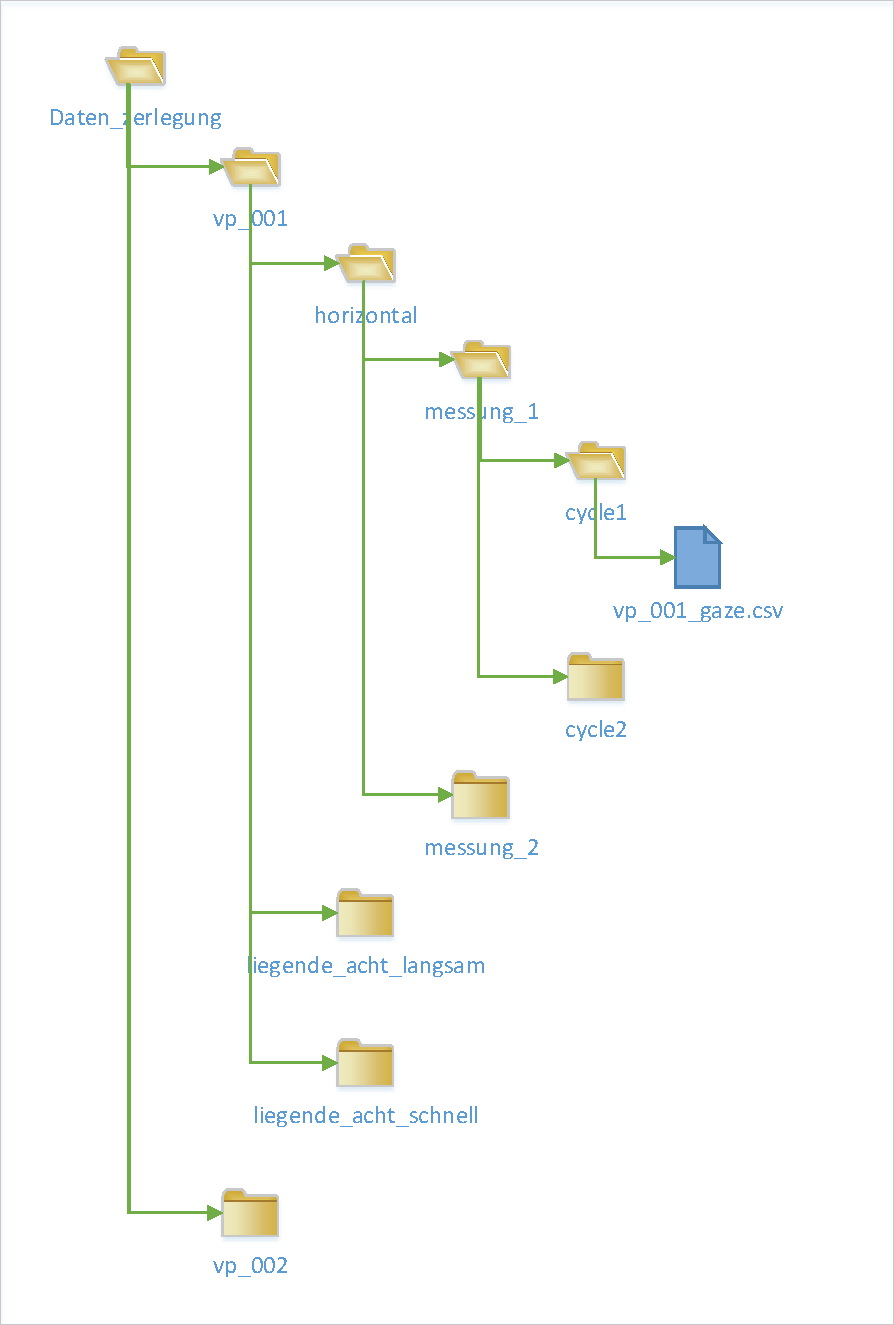
\includegraphics[width=15cm]{pics/Darstellung-Ordnerstruktur.pdf}
		\par\end{centering}
	\caption{\label{fig:Ordnerstruktur}Darstellung Ordnerstruktur}
\end{figure}

Die Versuche wurden dann visualisiert. \\
Durch die Visualisierung konnte man erkennen, dass die Targetdateien und die Blickdateien auf unterschiedlichen Koordinatensystemen beruhen. \\
Abbildung \ref{fig:Visualisierung} zeigt ein Beispiel f\"ur die Visualisierung der liegenden acht langsam.

\begin{figure}[H]
	\noindent \begin{centering}
		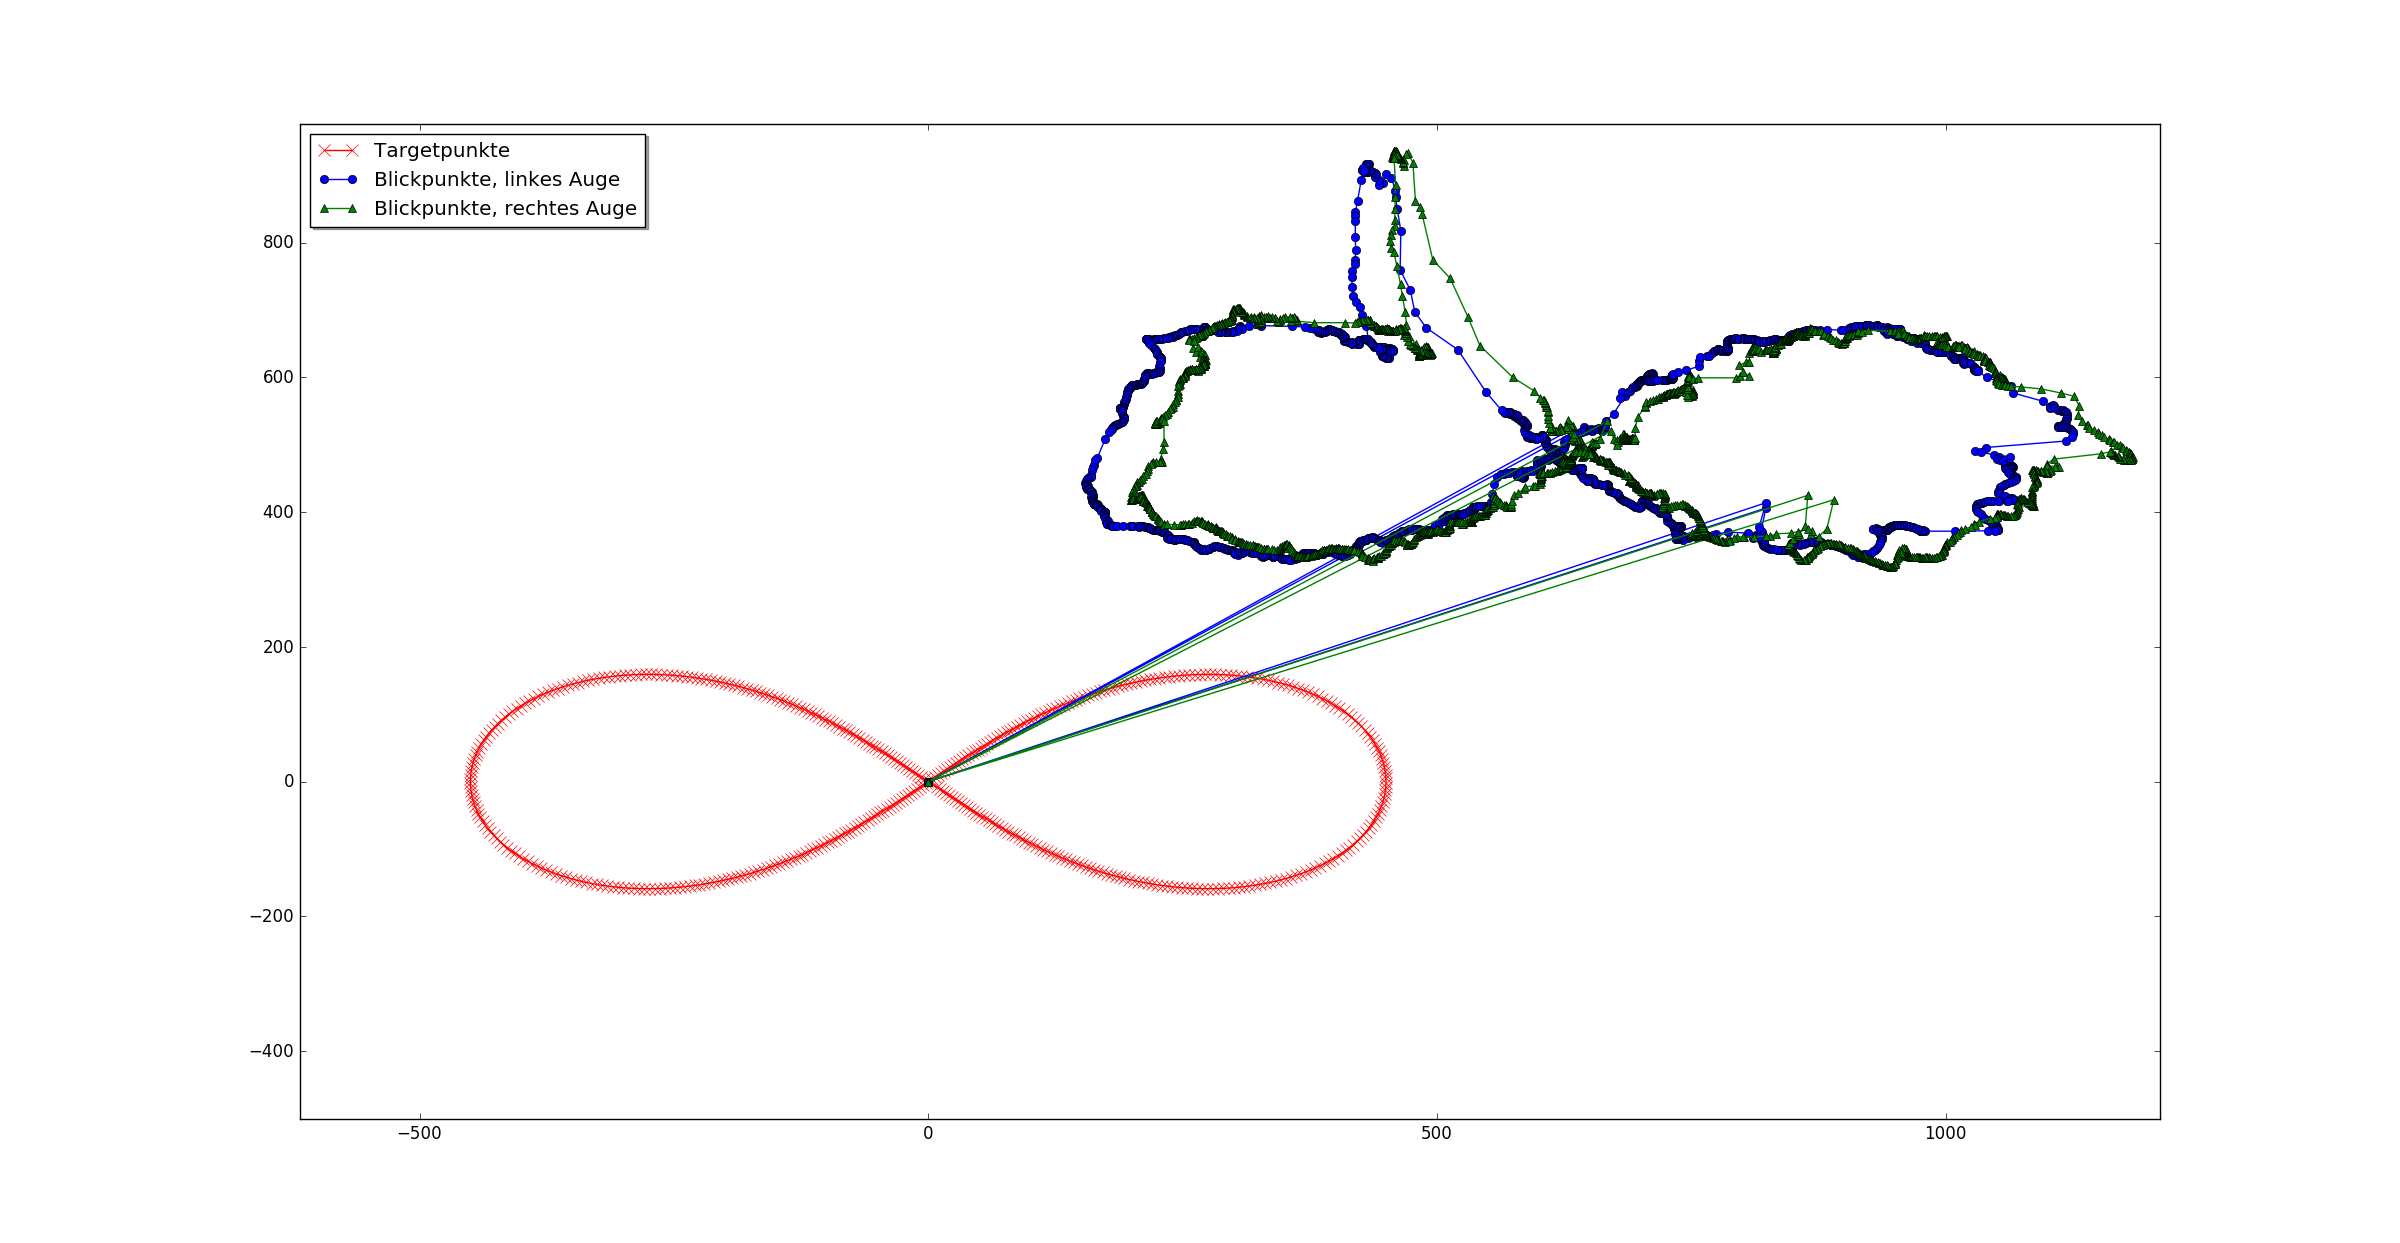
\includegraphics[width=15cm]{pics/figure_1-1.png}
		\par\end{centering}
	\caption{\label{fig:Visualisierung}Visualisierung der Blickpunkte}
\end{figure}
\chapter{Explorative Datenanalyse}
\chapter{Auff\"alligkeiten}
\begin{itemize}
	\item Bei den Daten ist bei Versuchsperson 131 aufgefallen, dass in der Targetdatei die Eintr\"age\\
		\textit{MSG:UserQuit:ProgramPaused}\\
		\textit{MSG:UserQuit:ProgramRestarted}
		\\ in der Spalte f\"ur den Zeitstempel vorkommen.
	
	\item Die Blickpunkte wurden mit drei- bis vierfacher Frequenz der Targetpunkte gemssen. \\
		Dadurch gibt es zwischen den Targetpunktmessungen mehrere Blickpunktmessungen.
	
	\item Es gibt in den Blickpunktdateien keinen Zeitstempel, der identisch ist mit dem aus einer dazugeh\"origen Targetpunktedatei. Dadurch erschwert sich die Zuordnung der Blickpunkte zu den Targetpunkten.
	
	\item In den Blickpunktdateien tritt oft der Fall auf, dass die x-Werte und die y-Werte f\"ur die Augen 0 sind.
	
	\item Fehlende Werte bei den Blickdateien wurden mit 0 kodiert. Diese treten mal f\"ur das linke und mal f\"ur das rechte Auge auf.
	
	\item Bei der Visualisierung hat sich gezeigt, dass der Koordinatenursprung bei den Blickdateien am linken oberen Rand des Bildschirms zu sein scheint, mit aufsteigenden Werten nach unten auf der Y-Achse und aufsteigenden Werten nach rechts auf der X-Achse. Das Koordinatensystem der Targetdateien liegt vermutlich im Mittelpunkt des Bildschirms mit aufsteigenden Werten nach oben auf der Y-Achse und aufsteigenden Werten nach rechts auf der X-Achse. Das l\"asst sich daraus ableiten, dass die Blickpunkte bei der Animation auf der Y-Achse immer in die entgegengesetzte Richtung zu der der Targetpunkte gingen. Auf der X-Achse stimmte die Richtung immer \"uberein.
	
	\item Die Blickdateien haben keine Headerzeile
	
	\item Die Zeitstempel sind nicht \"aquidistant
	
	\item Die Zeilenumbr\"uche in den Blickdateien, waren anders als die in den Targetdateien
	
	\item Blickpunkte wurden durchg\"angig gemessen, die Targetpunkte nur w\"ahrend der Versuche
	
	\item Einige Versuchspersonen haben nur Aufzeichnungen zu einem Auge (z.B. VP071)
	
	Da 3 Versuchspersonen besondere Auff\"alligkeiten vorzuweisen hatten, wurden diese nicht weiter verarbeitet. Das betrifft VP071 und VP090, da diese beiden nur mit einem Auge gemessen wurden, und VP131, da bei der Versuchsperson neu gestartet wurde.
	
\end{itemize}
\chapter{Fragen}
Aus den Auff\"ulligkeiten ergeben sich folgende Fragen:
\begin{enumerate}
	\item Welche Bedeutung haben die 0 Werte in den Blickdateien?
	
	Bedeuten diese, dass die Versuchsperson die Augen geschlossen hatte?
	\item Um welchen Wert sind die Koordinatensysteme verschoben?
	
	Gibt es eine Streckung des Koordinatensystems der Blickwerte zu dem der Targetwerte?
	\item K\"onnen wir davon ausgehen, dass die Zeitstempel der Blickdateien und der Targetdateien von synchron laufenden Uhren erstellt wurden?
	\item K\"onnen wir voraussetzen, dass der Fokus beim Sehen auf dem Mittelpunkt von der Blickposition des rechten und des linken Auges liegt?
\end{enumerate}
\chapter{Zusammenf\"uhrung der Daten}
Das Zusammenf\"uhren der Blickdaten und der Tagetdaten basiert auf den Zeitstempeln. Da die Blickdaten \"ofter gemessen wurden, als die Targetdaten und beim Verfolgen eines Punktes die Reaktion darstellen, wurde jedem Targetpunkt nur der Blickpunkt zugeordnet, der direkt nach dem Targetpunkt gemessen wurde. Alle weiteren Blickpunkte wurden verworfen.
\chapter{Merkmalserzeugung}
Bei der Merkmalserzeugung muss zwischen Merkmalen unterschieden werden, die innerhalb der Zeitreihen liegen und Merkmalen, die f\"ur die Gesamtbeschreibung der Versuchsperson genutzt werden.
\section{Abgeleitete Wertereihen}
Ein Merkmal innerhalb der Zeitreihen ist zum Beispiel die Mitte zwischen Blickposition des linken Auges und Blickposition des rechten Auges. Dabei wird f\"ur jeden Zeitpunkt im Datenstrom ein jeweiliger Wert berechnet.

Nachfolgend sind die Merkmale, die erzeugt werden k\"onnen aufgelistet.

\begin{table} [H]
	\caption{Merkmale innerhalb der Zeitreihe}
	\begin{tabular}[cc]{|l|l|}
		\hline
		\textbf{Merkmal} & \textbf{Berechnung}\\ \hline
		Mitte Augenpositionen & \begin{tabular}{c|c}
			$x=\frac{x_{links} + x_{rechts}}{2}$  & $y=\frac{y_{links} + y_{rechts}}{2}$ 
		\end{tabular} \\ \hline
		Abweichung Augenposition linkes Auge zu Targetpunkt & $s_l=\sqrt{{\left(x_{links}-x_{target}\right)}^2+{\left(y_{links}-y_{target}\right)}^2}$ \\ \hline
		Abweichung Augenposition rechtes Auge zu Targetpunkt & $s_r=\sqrt{{\left(x_{rechts}-x_{target}\right)}^2+{\left(y_{rechts}-y_{target}\right)}^2}$ \\ \hline
		Abweichung Mitte Augenposition zu Targetpunkt & $s_m=\sqrt{{\left(x_{mitte}-x_{target}\right)}^2+{\left(y_{mitte}-y_{target}\right)}^2}$ \\ \hline
		Geschwindigkeit linkes Auge & $v_l=\frac{\sqrt{{\left(x_{links_1}-x_{links_2}\right)}^2+{\left(y_{links_1}-y_{links_2}\right)}^2}}{\left(zeitstempel_1-zeitestempel_2 \right) }$ \\ \hline
		Geschwindigkeit rechtes Auge & $v_r=\frac{\sqrt{{\left(x_{rechts_1}-x_{rechts_2}\right)}^2+{\left(y_{rechts_1}-y_{rechts_2}\right)}^2}}{\left(zeitstempel_1-zeitestempel_2 \right) }$ \\ \hline
		Geschwindigkeit Mittelposition Augen & $v_m=\frac{\sqrt{{\left(x_{mitte_1}-x_{mitte_2}\right)}^2+{\left(y_{mitte}-y_{mitte}\right)}^2}}{\left(zeitstempel_1-zeitestempel_2 \right) }$ \\ \hline
		
	\end{tabular}
\end{table}
\section{Merkmale Versuchsperson}
\chapter{Clustern}

\newpage{}

\bibliographystyle{alphadin}
\clearpage\addcontentsline{toc}{chapter}{\bibname}\bibliography{bibtex/quellen}


\listoffigures


\listoftables

\end{document}
